\documentclass{standalone}
\usepackage{tikz,pgfplots,pgfplotstable}
\usepackage{xcolor}
\pgfplotsset{compat=newest}
\usetikzlibrary{positioning}
\usepgfplotslibrary{fillbetween}
\usetikzlibrary{shapes}

\newcommand{\smilename}{SMiLe$^{*}$}
\newcommand{\vsmile}{VarSMiLe}
\newcommand{\pfone}{pf1}
\newcommand{\pften}{pf10}
\newcommand{\pftwenty}{pf20}
\newcommand{\leaky}{Leaky}
\newcommand{\mpbayes}{Exact Bayes}
\newcommand{\mpone}{MP1}
\newcommand{\mpten}{MP10}
\newcommand{\mptwenty}{MP20}
\newcommand{\nassarten}{Nas10$^{*}$}
\newcommand{\nassartwelve}{Nas12$^{*}$}
\newcommand{\nassartenoriginal}{Nas10 original}
\newcommand{\nassartwelveoriginal}{Nas12 original}
\newcommand{\mporiginalone}{SOR1}
\newcommand{\mporiginalten}{SOR10}
\newcommand{\mporiginaltwenty}{SOR20}
\newcommand{\smileoriginal}{SMiLe}


\definecolor{mp1color}{rgb}{0.15,0.58,1}
\definecolor{mp10color}{rgb}{0,1,1}

\tikzset{
    %font = \scriptsize,
    font = \small,
    %font = \large,
    actualpcstyle/.style = {anchor = east, rotate = 90, isosceles triangle, fill = red!90!black, draw = none, inner sep = 1},
    mustyle/.style = {anchor = east, rotate = 90, isosceles triangle, fill = blue!80!black, draw = none, inner sep = 1, minimum width=0.3cm},
    smile/.style = {orange!90, thick},
    smileextended/.style = {red!60!black, thick},
    pf1/.style = {lime, thick},
    pf20/.style = {green!40!black, thick},
    leaky/.style = {gray, thick},
    bayesfilter/.style = {black, thick},
    gsor1/.style = {mp1color, thick},
    gsor20/.style = {blue, thick},
    tsor1/.style = {mp1color, thick},
    tsor10/.style = {mp10color, thick},
    tsor20/.style = {blue, thick},
    gnassarJN/.style = {magenta, thick},
    gnassarNatN/.style = {violet!90!black, thick},
    gnassarJNOriginal/.style = {magenta, thick, dashed},
    gnassarNatNOriginal/.style = {violet!90!black, thick, dashed},
    gsorOriginal1/.style = {green!95!black, thick},
    gsorOriginal20/.style = {mp10color, thick},
    tsorOriginal1/.style = {green!95!black, thick},
    tsorOriginal20/.style = {mp10color, thick},
    smileOriginal/.style = {orange!90, thick},
    %
    GNassarNatN_Sgmpositive/.style =  {orange!90, thick},
    GNassarNatN_Sgmnegative/.style =  {blue, thick},
    GNassarNatN_Sshpositive/.style =  {orange!90, thick},
    GNassarNatN_Sshnegative/.style =  {blue, thick},
    GParticleFilter_Sgmpositive/.style =  {orange!90, thick},
    GParticleFilter_Sgmnegative/.style =  {blue, thick},
    GParticleFilter_Sshpositive/.style =  {orange!90, thick},
    GParticleFilter_Sshnegative/.style =  {blue, thick},
    %
    GNassarNatN_Sgm/.style =  {green!40!black, thick},
    GNassarNatN_Ssh/.style =  {mp1color, thick},
    GParticleFilter_Sgm/.style =  {green!40!black, thick},
    GParticleFilter_Ssh/.style =  {mp1color, thick},
}
\pgfplotsset{
    legend style = {draw = none},
    colorbar/width = 6pt,
}
\newcommand{\plotwithquantiles}[2]{
    \addplot[draw = none, name path=lower] table[x = x, y expr = \thisrow{#1_mean} - \thisrow{#1_se}] {#2};
    \addplot[draw = none, name path=upper] table[x = x, y expr = \thisrow{#1_mean} + \thisrow{#1_se}] {#2};
    \addplot[#1, opacity = .4] fill between [of=lower and upper];
    \addplot[#1] table[x = x, y = #1_mean] {#2};
}
\newcommand{\trimleft}[1]{
    \begin{tikzpicture}[trim axis left]
        #1
    \end{tikzpicture}
}
\newcommand{\trimright}[1]{
    \begin{tikzpicture}[trim axis right]
        #1
    \end{tikzpicture}
}
\newcommand{\trimboth}[1]{
    \begin{tikzpicture}[trim axis right, trim axis left]
        #1
    \end{tikzpicture}
}
\newcommand{\heatmap}[2]{
    \begin{axis}[
        view = {0}{90},
        xtick = {-4,-3,-2.3,-2,-1.3,-1},
        xmin = -4.2, xmax = -.85,
        ymin = \ymin.2, ymax = .9,
        yticklabel = \empty,
        xticklabels = {$10^{-4}$,,,$10^{-2}$,},
        tick style = {white},
        xlabel = $p_c$,
        point meta min = -4., point meta max = \zmax,
        colormap/viridis,
        width = 4.8cm, height = 4.8cm,
        #2
        ]
        \addplot[matrix plot*, point meta = explicit, mesh/rows = \rows, mesh/cols = \cols]  table[x expr = log10(\thisrowno{1}),
              y expr = log10(\thisrowno{0}),
              meta expr = log10(\thisrowno{2})] {#1};
              \draw[white] (-4, \ymin.3) -- (-4, \ymin.05);
              \draw[white] (-2, \ymin.3) -- (-2, \ymin.05);
              \draw[white] (-4.3, -1) -- (-4.05, -1);
              \draw[white] (-4.3, 0) -- (-4.05, -0);
              \draw[white] (-4.3, -2) -- (-4.05, -2);
              \draw[white] (-4.3, .699) -- (-4.05, .699);
    \end{axis}
}

\newcommand{\heatmapblack}[2]{
    \begin{axis}[
      axis background/.style={fill=black},
        view = {0}{90},
        xtick = {-4,-3,-2.3,-2,-1.3,-1},
        xmin = -4.2, xmax = -.85,
        ymin = \ymin.2, ymax = .9,
        yticklabel = \empty,
        xticklabels = {$10^{-4}$,,,$10^{-2}$,},
        tick style = {white},
        xlabel = $p_c$,
        point meta min = -4., point meta max = \zmax,
        colormap/viridis,
        width = 4.8cm, height = 4.8cm,
        #2
        ]
        \addplot[matrix plot*, point meta = explicit, mesh/rows = \rows, mesh/cols = \cols]  table[x expr = log10(\thisrowno{1}),
              y expr = log10(\thisrowno{0}),
              meta expr = log10(\thisrowno{2})] {#1};
              \draw[white] (-4, \ymin.3) -- (-4, \ymin.05);
              \draw[white] (-2, \ymin.3) -- (-2, \ymin.05);
              \draw[white] (-4.3, -1) -- (-4.05, -1);
              \draw[white] (-4.3, 0) -- (-4.05, -0);
              \draw[white] (-4.3, -2) -- (-4.05, -2);
              \draw[white] (-4.3, .699) -- (-4.05, .699);
    \end{axis}
}

\usepackage{amsmath,amssymb}
\usetikzlibrary{calc}

\newcommand\xreference{0.4}
\newcommand\xstart{-2*\xreference - 0.5}
\newcommand\xstop{8*\xreference}

\newcommand{\approxs}[1]{\hat{#1}}
\newcommand\MUprior{0.}
\newcommand\SIGMAprior{0.8}
\newcommand\MUbeliefone{0.9}
\newcommand\SIGMAbeliefone{0.2}

\newcommand{\getY}[3]{exp(-(#1-#2)^2 / (2 * #3^2)) / (#3 * sqrt(2*pi))}

\newcommand\MUbelieftwo{2.1}
\newcommand\SIGMAbelieftwo{0.2}

\begin{document}

\begin{minipage}{19cm}
\centering
\begin{tabular}{l}
  \textbf{A} \\
    \hspace{30mm}
    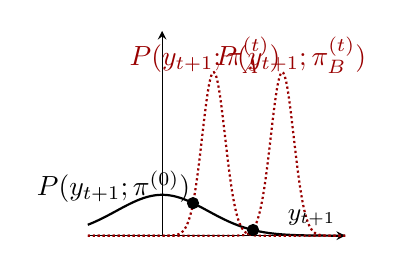
\begin{tikzpicture}
      \begin{axis}[
          name=axtaskdistr1,
          ytick=\empty,
          xtick=\empty,
          width = .4\textwidth,
          ymin = 0, ymax = 2.5,
          xlabel = $y_{t+1}$,
          axis lines=middle,
          clip=false,
          ]
          % density of Normal distribution:
          \addplot[black, thick, domain=\xstart:\xstop, samples=201]
                      {exp(-(x-\MUprior)^2 / (2 *\SIGMAprior^2))
                      / (\SIGMAprior * sqrt(2*pi))};
          \addplot[red!60!black, thick, densely dotted, domain=\xstart:\xstop, samples=201]
                      {exp(-(x-\MUbeliefone)^2 / (2 *\SIGMAbeliefone^2))
                      / (\SIGMAbeliefone * sqrt(2*pi))};
          \addplot[red!60!black, thick, densely dotted, domain=\xstart:\xstop, samples=201]
                      {exp(-(x-\MUbelieftwo)^2 / (2 *\SIGMAbelieftwo^2))
                      / (\SIGMAbelieftwo * sqrt(2*pi))};
          \addplot[black, mark=*] coordinates {(\MUbeliefone - 0.36,\getY{\MUbeliefone - 0.36}{\MUprior}{\SIGMAprior})}{} ;
          \addplot[black, mark=*] coordinates {(\MUbelieftwo - 0.51,\getY{\MUbelieftwo - 0.51}{\MUprior}{\SIGMAprior})}{} ;
          % Text and lines
          \node[font={\fontsize{10pt}{12 pt}\selectfont}] at (axis cs: -0.85,0.6) {$P(y_{t+1}; \pi^{(0)})$};
          \node[font={\fontsize{10pt}{12 pt}\selectfont}, color=red!60!black] at (axis cs: \MUbeliefone - 0.15, 2.2) {$P(y_{t+1}; \pi_A^{(t)})$};
          \node[font={\fontsize{10pt}{12 pt}\selectfont}, color=red!60!black] at (axis cs: \MUbelieftwo + 0.15, 2.2) {$P(y_{t+1}; \pi_B^{(t)})$};
        \end{axis}
    \end{tikzpicture}
    \vspace{10pt}
    \\
    \begin{tabular}{ll}
    \textbf{B} \hspace{25mm} \nassartwelve & \hspace{32mm} \pftwenty\\
    \hspace{4pt}
    \begin{tikzpicture}
        \pgfplotstableread{../data_final/experiment_second_20subj_500steps/exp_second_GNassarNatNsigma0.5_pc0.1_steps500_Dp0.0125.csv}\data
        \begin{axis}[
            width = .32\textwidth,
            xmax = 0.36,
            grid = both,
            ylabel = $\Bar{\textbf{S}}$,
            xlabel = $p$]
            \plotwithquantiles{GNassarNatN_Sgm}{\data}
            \plotwithquantiles{GNassarNatN_Ssh}{\data}
        \end{axis}
    \end{tikzpicture}
               &
    \hspace{10pt}
    \begin{tikzpicture}
        \pgfplotstableread{../data_final/experiment_second_20subj_500steps/exp_second_GParticleFiltersigma0.5_pc0.1_steps500_Dp0.0125.csv}\data
        \begin{axis}[
            width = .32\textwidth,
            xmax = 0.36,
            grid = both,
            ylabel = $\Bar{\textbf{S}}$,
            xlabel = $p$,
            legend to name = experimentsecondfigurelegend,
            legend entries = {,,,$\Bar{\textbf{S}}_{\mathrm{BF}}$,,,,$\Bar{\textbf{S}}_{\mathrm{Sh}}$},
            legend columns = 1]
            \plotwithquantiles{GParticleFilter_Sgm}{\data}
            \plotwithquantiles{GParticleFilter_Ssh}{\data}
        \end{axis}
    \end{tikzpicture}
    \\
    & \multicolumn{1}{r}{\ref{experimentsecondfigurelegend}}
\end{tabular}
\end{tabular}

\end{minipage}
\end{document}
